\subsection{Parámetros auditados}

\texttt{scripts/pacca/measure\_warmup.py} determina el intervalo de
calentamiento de cada kernel mediante un umbral de coeficiente de variación
(CV\%) sobre una señal de carga (IPC en CPU, utilización de GPU reportada
por NVML en GPU), con un método de respaldo por detección de puntos de
cambio cuando el umbral de CV no encuentra un punto estable. Cinco
constantes internas de este procedimiento se auditan aquí:
\texttt{CV\_THRESHOLD\_PCT} (umbral de CV, actualmente 5\,\%),
\texttt{MARGIN} (margen de seguridad multiplicativo sobre el punto
detectado, actualmente $\times 1.2$), \texttt{min\_mean\_floor} (piso de
ruido para señales de GPU, actualmente 5{,}0\,\% de utilización),
\texttt{plateau\_ratio} (fracción de la meseta de mayor carga que debe
alcanzar un segmento para aceptarse como fin del calentamiento en el
método de respaldo, actualmente 0{,}8) y los parámetros internos de
segmentación (\texttt{min\_relative\_gain}, \texttt{max\_depth}).

A diferencia de los demás barridos de este informe, este no requirió
cómputo nuevo en \texttt{paccaA100}: se reprocesaron las trazas crudas ya
recolectadas durante la caracterización del catálogo (tres kernels GPU con
transición de carga real -- \texttt{rodinia\_hotspot}, \texttt{rodinia\_heartwall},
\texttt{rodinia\_lavamd} -- y tres kernels CPU con fases conocidas --
\texttt{npb\_bt}, \texttt{npb\_cg}, \texttt{rodinia\_lud}), variando cada
parámetro dentro de un rango razonable mientras los demás se mantienen en
su valor por defecto.

\subsection{Piso de ruido GPU (\texttt{min\_mean\_floor}): justificación por punto de inflexión}

La Figura~\ref{fig:sens-floor} muestra el hallazgo más claro de este
barrido: para los tres kernels GPU con transición de carga real, el
calentamiento detectado es \textbf{0 o casi 0 cuando el piso de ruido está
en 0 o 2\,\%}, y se estabiliza en el valor físicamente correcto (confirmado
contra la traza cruda de potencia en el catálogo, ARC-86) en 5\,\%, 8\,\%
y 12\,\% -- los tres dan el mismo resultado. El rango probado
(0, 2, 5, 8, 12\,\%) tiene un salto de 3 puntos porcentuales entre el
último valor degenerado (2\,\%) y el primer valor estable (5\,\%): esto
demuestra que el punto de inflexión real está \emph{en algún lugar dentro
de ese intervalo (2, 5]\,\%}, y que 5\,\% ya está del lado correcto con
margen (comparte resultado con 8\,\% y 12\,\%, muy por encima del umbral),
pero \textbf{no} que 5\,\% sea, cifra exacta, el punto de inflexión --
eso requeriría un barrido más fino entre 2\,\% y 5\,\% (por ejemplo, cada
0{,}5 puntos) que no se hizo aquí. Lo que sí puede afirmarse sin matices:
por debajo de ese intervalo, el detector cae en el modo de falla original
que motivó introducir este parámetro (una ventana de utilización cercana a
cero se declara ``estable'' por construcción del coeficiente de
variación), y 5\,\% está de forma demostrada e inequívoca del lado
correcto, con margen de sobra hasta 12\,\%.

\begin{figure}[H]
\centering
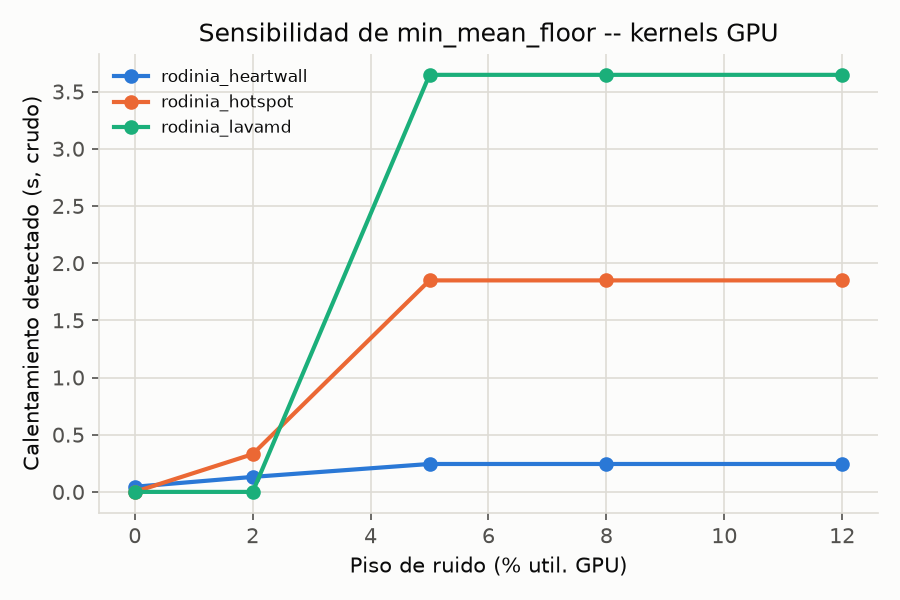
\includegraphics[width=0.85\textwidth]{../plots/warmup_sensitivity/sensitivity_min_mean_floor_gpu.png}
\caption{Calentamiento detectado en función del piso de ruido GPU, para los
tres kernels con transición de carga real. La meseta a partir de 5\,\%
confirma que el valor actual está del lado correcto y con margen del
punto de inflexión (ubicado en algún punto del intervalo (2,5]\,\%, no
resuelto con mayor precisión aquí).}
\label{fig:sens-floor}
\end{figure}

\subsection{Umbral de CV\% (\texttt{CV\_THRESHOLD\_PCT}): robusto en la mayoría de los casos, con una excepción real}

Georges, Buytaert y Eeckhout \citep{Georges2007} recomiendan un umbral de
1--2\,\% para este método; conviene precisar que ese umbral se estableció
para la máquina virtual de Java (variabilidad introducida por JIT y
recolector de basura), un contexto distinto al de un kernel HPC nativo sin
capas de gestión en tiempo de ejecución, así que se cita como antecedente
metodológico del propio método de detección de calentamiento por CV\%, no
como una recomendación directamente transferible al valor numérico usado
aquí. El proyecto usa 5\,\% (heredado del chequeo de estabilidad de
referencia CAL-10, no de la literatura). La
Figura~\ref{fig:sens-cv} muestra el resultado de barrer el umbral entre
1\,\% y 10\,\% sobre los seis kernels:

\begin{itemize}
  \item \texttt{rodinia\_hotspot}, \texttt{rodinia\_heartwall},
    \texttt{rodinia\_lavamd} y \texttt{npb\_bt} son \textbf{completamente
    robustos} en todo el rango 1--10\,\%: el punto detectado no cambia en
    absoluto.
  \item \texttt{npb\_cg} es robusto entre 1\,\% y 8\,\%, pero a 10\,\% la
    detección colapsa a 0\,s (falso positivo) -- evidencia de que el
    umbral no puede subirse indefinidamente sin reintroducir el modo de
    falla, aunque 5\,\% conserva margen de sobra frente a ese límite.
  \item \texttt{rodinia\_lud} es el caso genuinamente sensible: el punto
    detectado se mueve de 0{,}230\,s (8--10\,\%) a 0{,}268\,s (5\,\%) a
    0{,}290\,s (2\,\%), y a 1\,\% el criterio de CV ya no encuentra ningún
    punto y cae al método de respaldo. La variación relativa entre 2\,\% y
    8\,\% es de apenas 0{,}06\,s sobre una corrida de $\sim$12\,s -- no
    altera ninguna conclusión práctica, pero es la evidencia honesta de que
    no todos los kernels son igual de robustos a esta elección.
\end{itemize}

\begin{figure}[H]
\centering
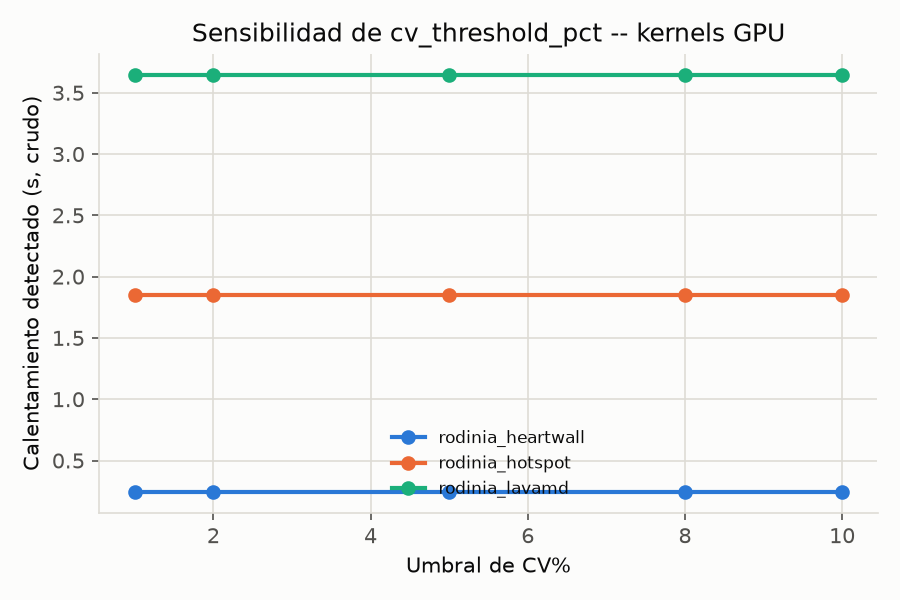
\includegraphics[width=0.85\textwidth]{../plots/warmup_sensitivity/sensitivity_cv_threshold_pct_gpu.png}
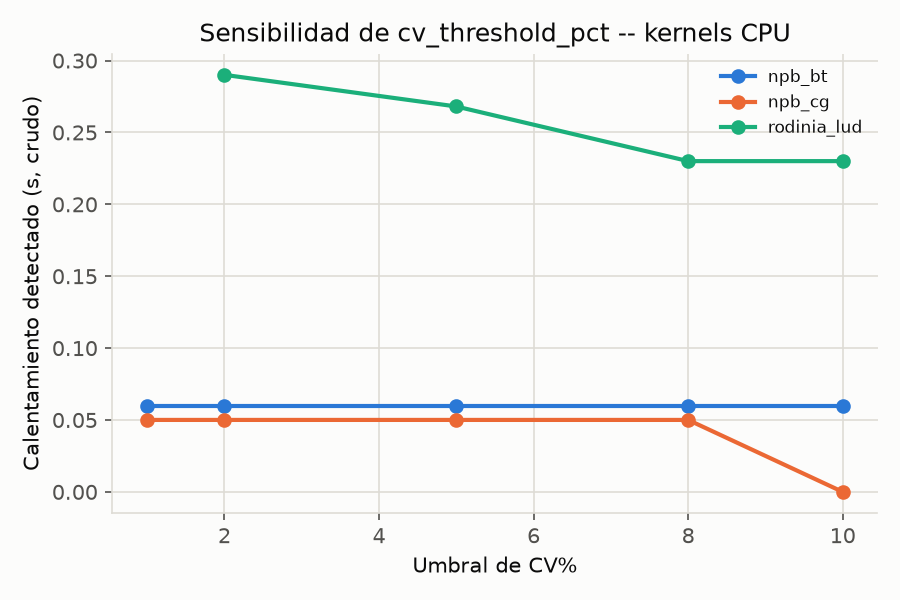
\includegraphics[width=0.85\textwidth]{../plots/warmup_sensitivity/sensitivity_cv_threshold_pct_cpu.png}
\caption{Calentamiento detectado en función del umbral de CV\%, kernels GPU
(arriba) y CPU (abajo). La mayoría de las líneas son planas (robustas); la
de \texttt{rodinia\_lud} tiene pendiente real, y la de \texttt{npb\_cg} cae
a cero en el extremo derecho.}
\label{fig:sens-cv}
\end{figure}

\textbf{Conclusión}: el umbral de 5\,\% queda confirmado como una elección
segura -- ni tan bajo como para perder detección en \texttt{rodinia\_lud},
ni tan alto como para caer en el falso positivo de \texttt{npb\_cg} a
10\,\% -- pero su origen (``prestado'' de CAL-10, no derivado
independientemente) sigue sin una justificación de primer principio más
allá de esta verificación empírica de robustez.

\subsection{Margen de seguridad (\texttt{MARGIN})}

El margen es, por construcción, una función lineal del punto crudo
detectado ($t_{\text{propuesto}} = t_{\text{crudo}} \times \text{margen}$),
así que no hay una relación no trivial que descubrir aquí -- la
Figura~\ref{fig:sens-margin} simplemente cuantifica cuántos segundos
representa cada opción de margen para los kernels reales. Para
\texttt{rodinia\_lavamd}, el kernel con mayor calentamiento absoluto, la
diferencia entre no aplicar margen ($\times 1.0$) y el valor actual
($\times 1.2$) es de 0{,}73\,s; para \texttt{npb\_cg}, de apenas 0{,}01\,s.
No se encontró evidencia de que $\times 1.2$ sea insuficiente o excesivo en
ningún caso real -- la elección permanece una decisión de ingeniería
razonable sin una derivación estadística propia (por ejemplo, a partir de
la varianza del punto detectado entre repeticiones), que queda como
mejora futura.

\begin{figure}[H]
\centering
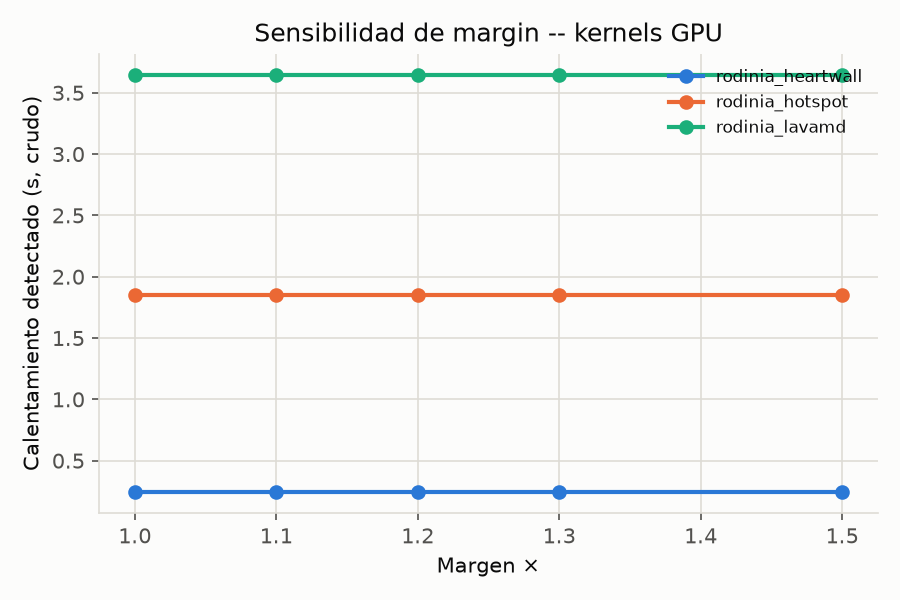
\includegraphics[width=0.85\textwidth]{../plots/warmup_sensitivity/sensitivity_margin_gpu.png}
\caption{Calentamiento propuesto (crudo × margen) en función del margen de
seguridad, kernels GPU.}
\label{fig:sens-margin}
\end{figure}

\subsection{Fracción de meseta (\texttt{plateau\_ratio})}

Ninguno de los seis kernels de esta muestra activó el método de respaldo
por punto de cambio con sus parámetros por defecto (todos se resolvieron
por el umbral de CV), así que este barrido no pudo ejercitar
\texttt{plateau\_ratio} con datos reales de este proyecto -- las líneas son
planas en el rango 0{,}6--0{,}9 simplemente porque el método de respaldo
nunca se invocó. La justificación de 0{,}8 sigue siendo, por tanto, la
descrita en ARC-86 (corrige un modo de falla real observado en
\texttt{rodinia\_hotspot} durante su caracterización), no una verificada
por barrido de sensibilidad en este documento. \textbf{Pendiente}: repetir
este barrido específicamente sobre un kernel que sí caiga en el método de
respaldo (por ejemplo, forzando \texttt{CV\_THRESHOLD\_PCT} a un valor muy
bajo para inducir el respaldo de forma controlada) antes de considerar este
parámetro completamente verificado.
